In this exercise we will explore a container of volume $V$ with $N$ rod-shaped particles which all can change their orientation to be along one of the coordinate axes. $N_i$ denotes the number of particles oriented in direction $i$. The temperature $T$ (including the Boltzmann constant) of the system is held constant. The Helmhotz fre energy of the system is given in \cref{eq:helm}.
\begin{equation}
    F=T\left[N_x \ln \left(\alpha \frac{N_x}{V}\right)+N_y \ln \left(\alpha \frac{N_y}{V}\right)+N_z \ln \left(\alpha \frac{N_z}{V}\right)+\gamma \frac{N_x N_y+N_y N_z+N_z N_x}{V}\right]
    \label{eq:helm}
\end{equation}


\subsection*{a)}
    To find an expression for entropy of our system we use the derivative of Helmholtz free energy $dF = -SdT - PdV + \mu dN$, giving 
    \begin{align}
        S =& - \pclosed{\pdv{F}{T}}_{V, N}\\
         =& -\left[ N_x \ln \left(\alpha \frac{N_x}{V}\right)+N_y \ln \left(\alpha \frac{N_y}{V}\right)+N_z \ln \left(\alpha \frac{N_z}{V}\right)+\gamma \frac{N_x N_y+N_y N_z+N_z N_x}{V} \right]
    \label{eq:entropy}
    \end{align}
    as the expression of entropy.


\subsection*{b)}
    To examine our system we look into which concentrations of the different rod-orientations are present when we increase our overall concentration $n = \frac{N}{V}$. We start our system at a low consentration and examine it as we slowly increase the number rods while keeping $V$ and $T$ constant resulting in an increase in concentration. We refer to the concentrations of rods in the different orientations as $n_x, n_y$ and $n_z$. This gives the new expression for Helmhotz free energy in \cref{eq:helm_new}.   
    \begin{equation}
        F=TV\left[n_x \ln \left(\alpha n_x\right)+n_y \ln \left(\alpha n_y\right)+n_z \ln \left(\alpha n_z\right)+\gamma (n_x n_y+n_y n_z+n_z n_x)\right]
        \label{eq:helm_new}
    \end{equation}
    We notice that $V$ is now just a scaling of $F$.

    For each $n$ we can find an $n_x, n_y$, and $n_z$ which minimise the system's energy, and according to the energy minimum principle the system will naturally employ these values when the entropy is being held constant (as it will be for each $N$, see \cref{eq:entropy}). We implement the numerical tool scipy.minimise to find the concentrations yielding the lowest $F$. In this case our system has two constraints:
    \begin{enumerate}
        \item $n_x + n_y + n_z = n$
        \item $ N<V  \Rightarrow \frac{N}{V} = n < 1$
    \end{enumerate}

    When plotting the different concentrations as functions of the total concentration we get the plot shown in \cref{fig:n_vs_xyz}. 
    \begin{figure}
        \centering
        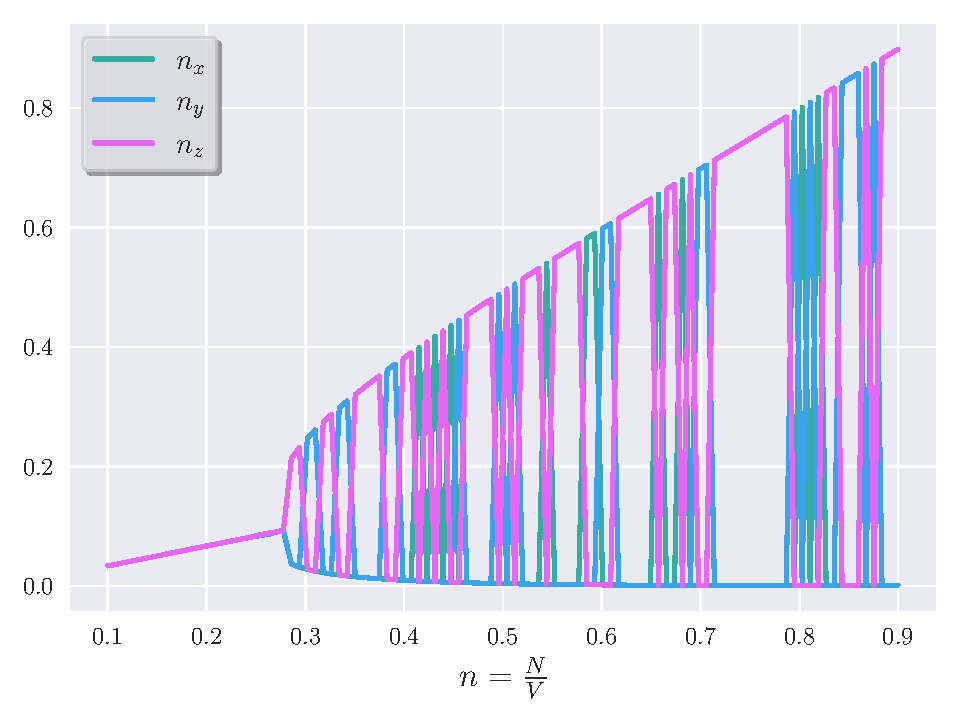
\includegraphics[width=.7\textwidth]{./figs/n_vs_xyz.pdf}
        \caption{Plot of the concentrations of different rod-orientations which minimise $F$, as functions of the total concentration.}
        \label{fig:n_vs_xyz}
    \end{figure}
    
    From this we can see that for small $n$, $n_x=n_y=n_z$. However, around $n \geq 0.3$ the concentrations diverge and alternate bewteen being large and small. This points to something happening to our system around this concentration. To further analyse this, we plot the minimised Helmhotz free energy as a function of $n$, see \cref{fig:n_vs_F}.    
    \begin{figure}
        \centering
        \begin{subfigure}[b]{0.49\textwidth}
            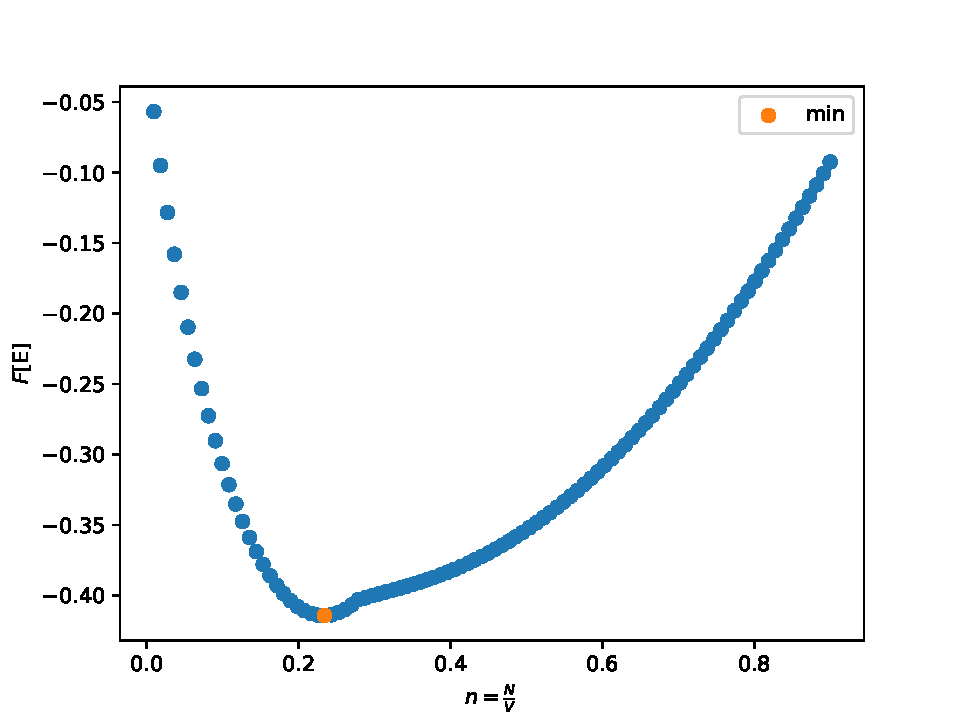
\includegraphics[width=\textwidth]{./figs/n_vs_F.pdf}
            \caption{The minimised Helmholtz free energy as a function of the total concentration.}
            \label{fig:n_vs_F_a}
        \end{subfigure}
        \begin{subfigure}[b]{0.49\textwidth}
            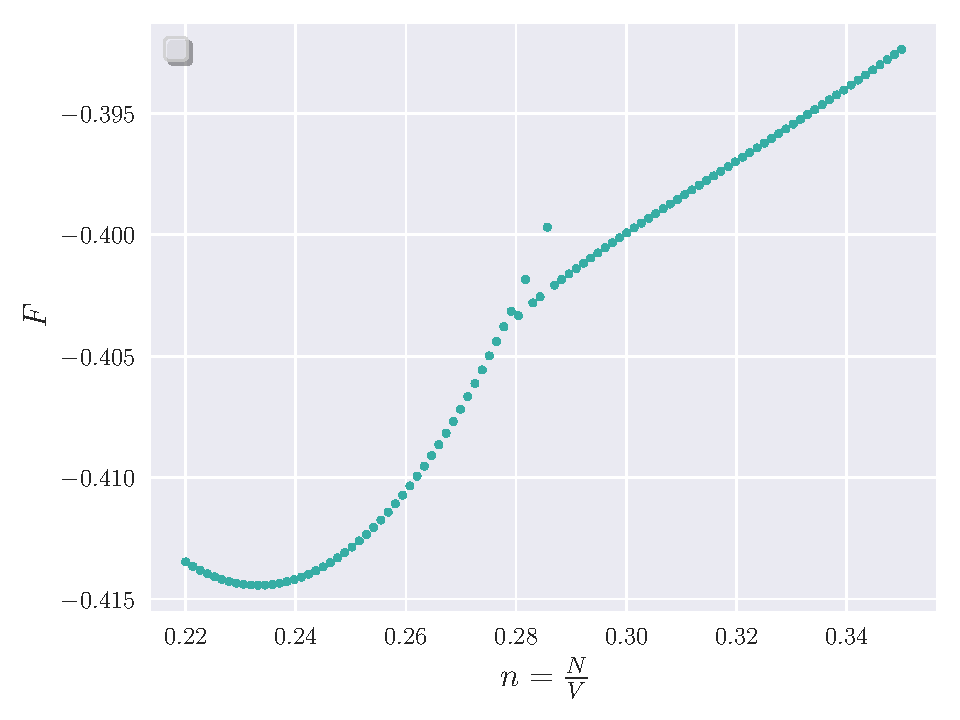
\includegraphics[width=\textwidth]{./figs/n_vs_F_zoomed.pdf}
            \caption{\cref{fig:n_vs_F_a} zoomed in on the region of discontinuity.\linebreak}
        \end{subfigure}
        \caption{}
        \label{fig:n_vs_F}
    \end{figure}
    There we can see that $F$ has a discontinuity around $n = 0.28$. In addition the $\pdv{^2F}{n^2} < 0$ around the same point, signalling some instability in the system. On both sides of this interval however, the system is stable ($\pdv{^2F}{n^2} > 0$). 
    
    Lastly, we will look at some contour plots of $F$ for constant $n$ with different rod-orientations-concentrations, see \cref{fig:cont}. These plots visualise the various $n_x, n_y$, and $n_z$ which minimise the energy. 
    \begin{figure}
        \centering
        \begin{subfigure}[b]{0.49\textwidth}
            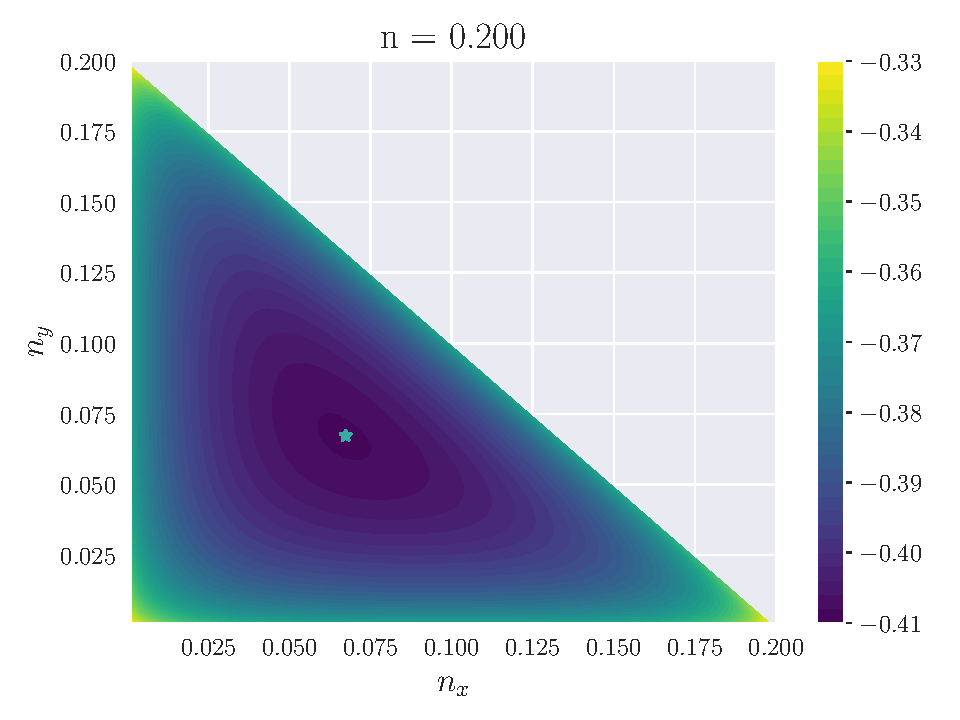
\includegraphics[width=\textwidth]{./figs/contour_nan_0.2.pdf}
            \caption{Small total concentration. One minimum where $n_x = n_y = n_z$}
        \end{subfigure}
        \begin{subfigure}[b]{0.49\textwidth}
            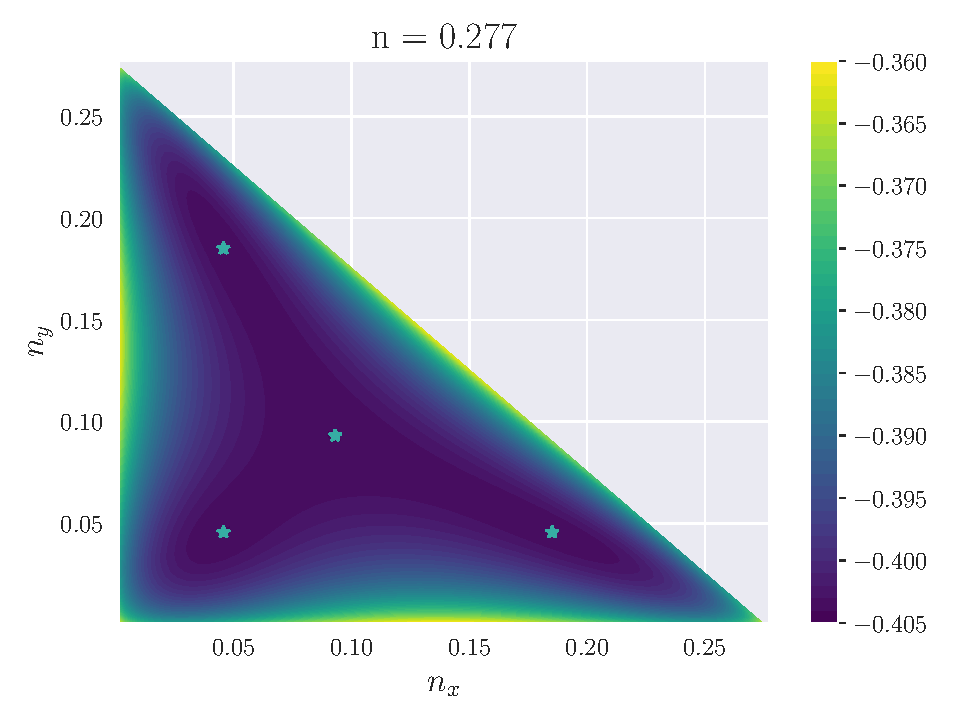
\includegraphics[width=\textwidth]{./figs/contour_nan_0.2773.pdf}
            \caption{Four minima, pointing towards coexistence of phases .}
        \end{subfigure}
        \begin{subfigure}[b]{0.49\textwidth}
            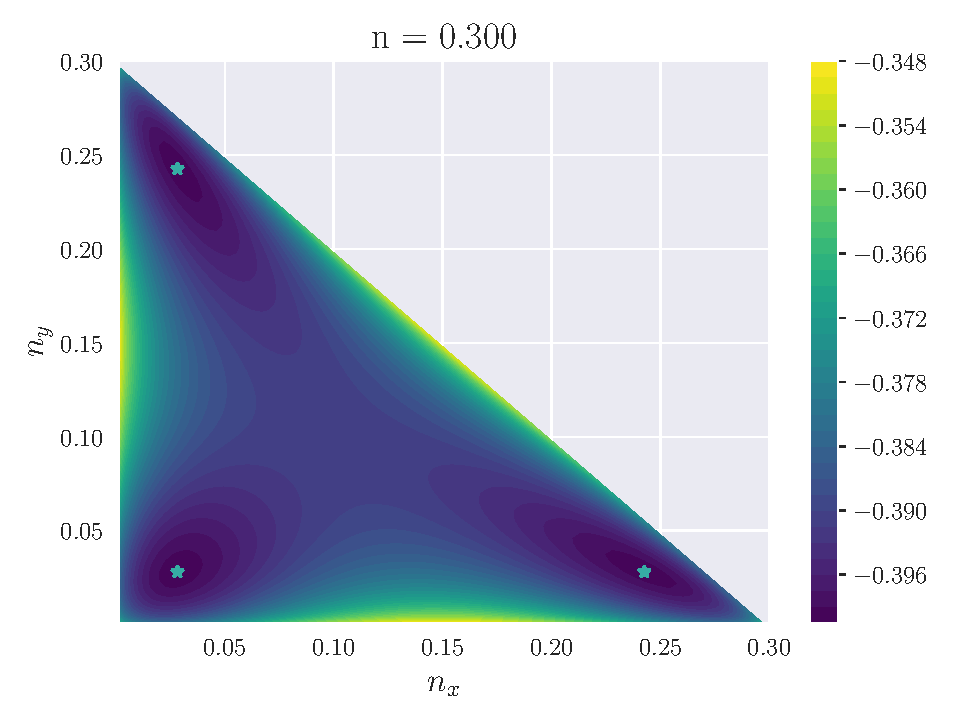
\includegraphics[width=\textwidth]{./figs/contour_nan_0.3.pdf}
            \caption{Three minima; one concentration domintaing. \linebreak }
        \end{subfigure}
        \begin{subfigure}[b]{0.49\textwidth}
            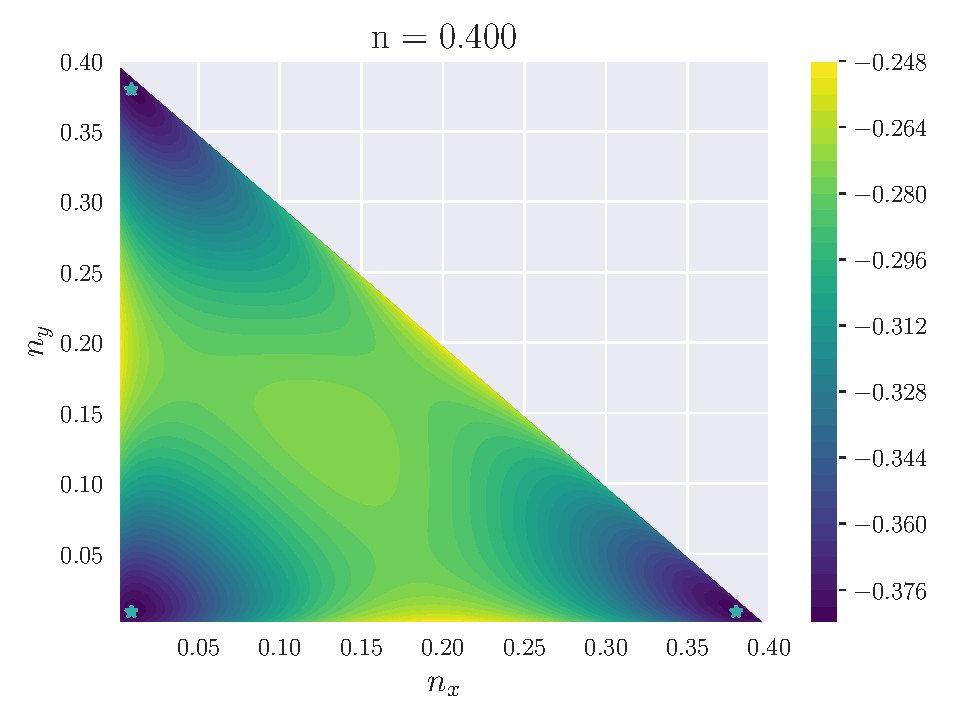
\includegraphics[width=\textwidth]{./figs/contour_nan_0.4.pdf}
            \caption{Three minima; one concentration domintaing. Now the previous minimum, $n_x = n_y = n_z$, is a maximum. }
        \end{subfigure}
        \caption{Contour plots of F vs $n_x$ and $n_y$. The blue stars show the minima. $n_z$ is not depicted, but can in each point of the plot be deducted by taking $n_z = n - n_x - n_y$.}
        \label{fig:cont}
    \end{figure}  
    Analysing the plots in \cref{fig:cont}. When $n=0.2$ the point minimising the energy is $n_x = n_y = n_z$, a results which corresponds with the plot in \cref{fig:n_vs_xyz}. However, when $n=0.277$ we see that there are four minima; one where the rod-concentrations are all equal, and three where each one of them dominates. When further increasing $n$, the minima only consist of the ones with one increasingly dominant rod-direction. When $n=0.4$ we see that the point where they are all equal has now become a maximum. 

    All the obtained results point to the same conclusion: there seems to be an interval of concentrations which corresponds to a phase of coexistence, and on either side of this interval we have a stable phase; meaning the system undergoes a phase transition. One phase is when the rod-concentrations are all equal (disordered phase), and the other when one orientation dominates (ordered phase). Ananlysing the system energy, one can see that at low concentrations, the system benefits from being in the disordered phase, and when the concentration is increased beyond a certain point (around $n=0.3$) the system benefits from being in a more ordered phase. The contour plot where $n=0.277$ shows the coexistence of these two phases. As does the plot in \cref{fig:n_vs_F}, where the double derivative of $F$ is negative. The concentration intervals across the plots coincide supporting the hypothesis.  



\subsection*{c)}
    Now we would like examine our system while keeping $N$ (and $T$) constant and increasing the pressure, $P$, by decreasing the volume, $V$. As $n = \frac{N}{V}$, decreasing the volume, while keeping $N$ constant, will be similar to increasing the concentration. Earlier we found which combination of $n_x, n_y,$ and $n_z$ equal to a certain $n$ minimized the system energy. We now want to find which combination of $n_x, n_y,$ and $n_z$ for a certain $V$ minimize the energy. We then want to look at the system energy as a function of changing $P$. 
    
    To find the optimal combination of $n_x, n_y,$ and $n_z$ for a certain $V$, we can still minimize the Helmholtz free energy. That means we will have the same rod-concentrations as a function of total concentration as before (ref \cref{fig:n_vs_xyz}), and our system will undergo the same changes. However, when we want to plot the system energy as a function of $P$, we have to look at an energy which depends on $P$ ($F$ is a function of $T, V,$ and $N$), like Gibbs free energy. The relation between $F$ and $G$ is:
    \begin{equation}
        G = F + PV
    \end{equation} 
    To find $G$ we need to find an expression of $P$ as a function of our known variables. To do this we implement the relation $dF = -S dt - P dV$, giving:
    \begin{equation}
        P = -\pclosed{\pdv{F}{V}}_{T,N} = - T \bclosed{n_x + n_y + n_z + \gamma (n_x n_y + n_y n_z + n_z n_x)}
    \end{equation}
    
    Plotting our results of $G$ as a function of $P$ gives the plot in figure \cref{fig:gibbs}
    \begin{figure}
        \centering 
        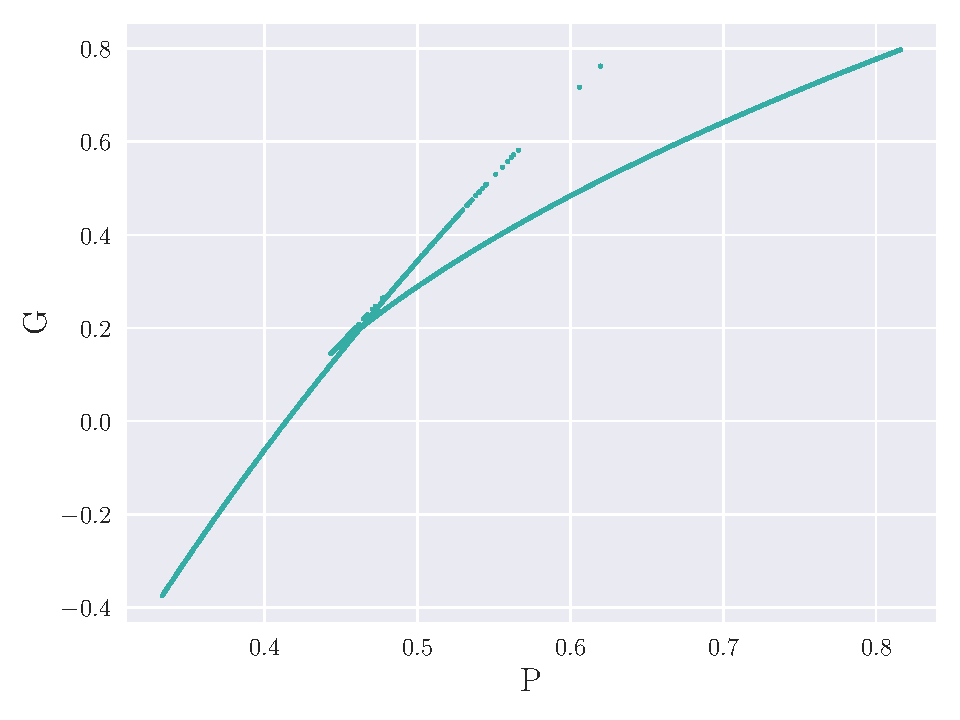
\includegraphics[width=.7\textwidth]{./figs/gibbs.pdf}
        \caption{Plot of Gibbs free energy as a function of pressure. The graph overlaps with itself resulting in one value of pressure yielding several values of energy.}
        \label{fig:gibbs}
    \end{figure}
    We can see that around $P=0.47$ the function crosses itself, much like shown in Figure 17.3 in the textbook. This point is referred to as the critical pressure of the system, and the graph's overlap can be explained by the coexistence of phases. 
    
    To futher analyse this coexistence, we plot the pressure as a function of $n$, see \cref{fig:n_vs_P}. 
    \begin{figure}
        \centering 
        \begin{subfigure}[b]{0.49\textwidth}
            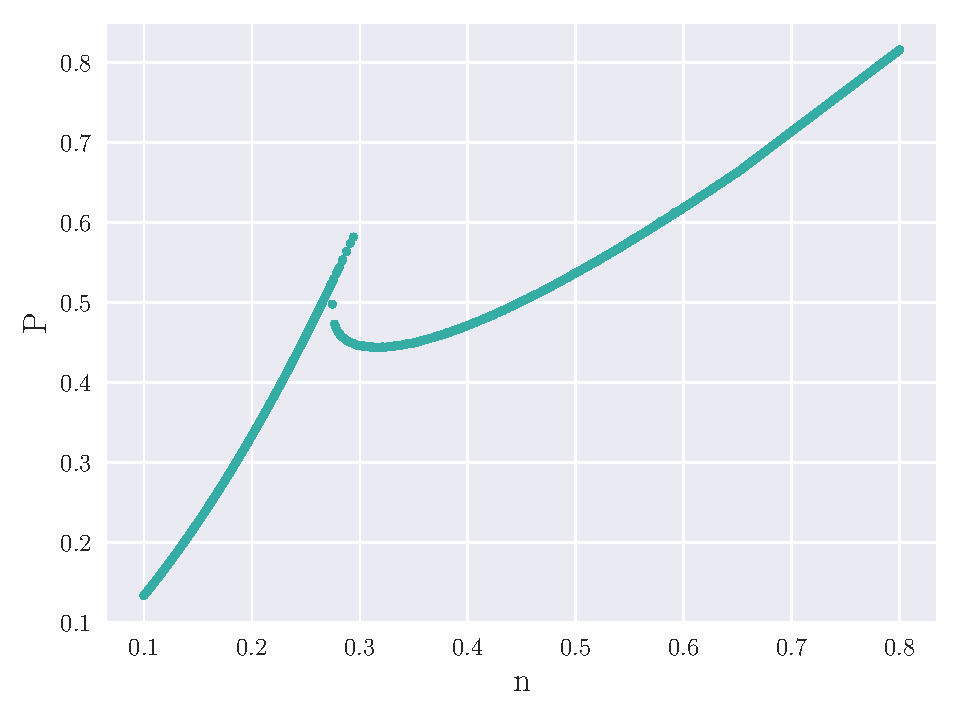
\includegraphics[width=\textwidth]{./figs/n_vs_P.pdf}
            \caption{}
            \label{fig:n_vs_P_a}
        \end{subfigure}
        \begin{subfigure}[b]{0.49\textwidth}
            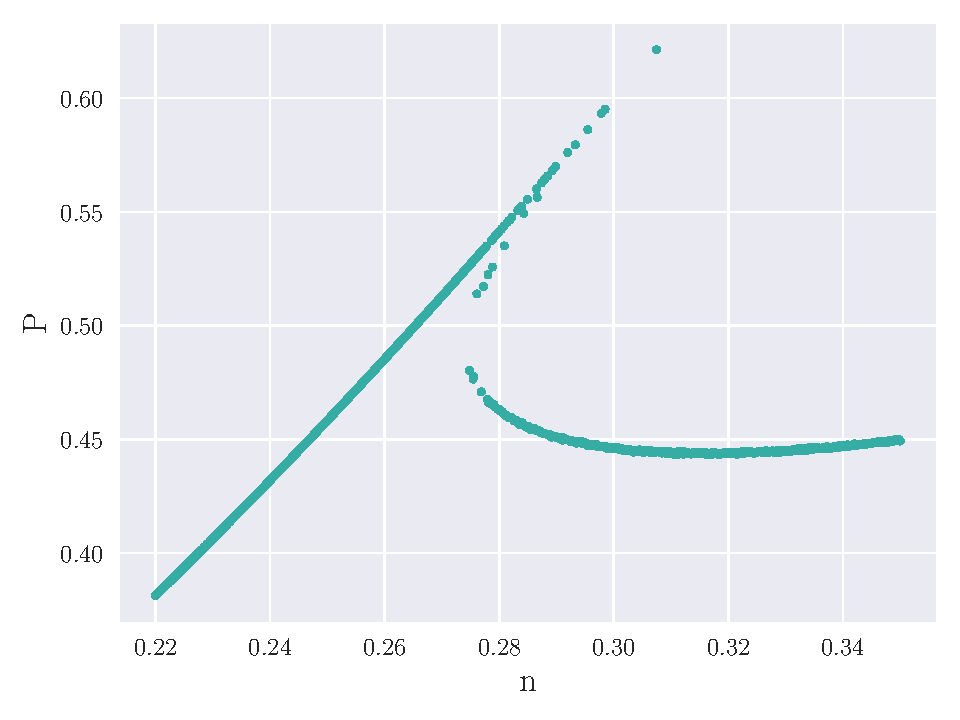
\includegraphics[width=\textwidth]{./figs/n_vs_P_zoom.pdf}
            \caption{\cref{fig:n_vs_P_a} zoomed in on the area of discontinuity.}
        \end{subfigure}
        \caption{Plot of pressure as a function of total concentration.}
        \label{fig:n_vs_P}
    \end{figure}
    In the last exercise we saw a concentration interval in which our results indicated a coexistence of phases. Now, we see that in the same interval there exist multiple $P$ values for each $n$. As different phases have different pressures we have again found an indication of coexistence of phases in our system. 


